%%%%%%%%%%%%%%%%%%%%%%%%%%%%%%%%%%%%%%%%%%%%%%%%%%%%%%
%%%%%%%%%%%%%%%%%%%%%%%%%%%%%%%%%%%%%%%%%%%%%%%%%%%%%%
\section[Model based optim.]{Model based optimization methods}
\subsection{}

%%%%%%%%%%%%%%%%%%%%%%%%%%%%%%%%%%%%%%%%%%%%%%%%%%%%%%
\begin{frame}{}
If the number of function evaluations are limited, we can run the optimization on the model instead of running it directly on the function
\begin{center}
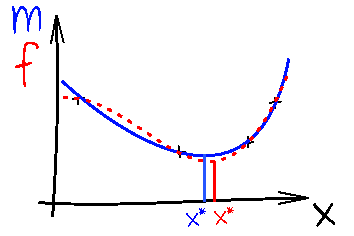
\includegraphics[height=5cm]{4_optimization/figures/ink_mf}
\end{center}
In the end, we hope that:
\begin{equation*}
	\begin{split}
		\argmin(m) & \approx \argmin(f)\\
		\min(m) & \approx \min(f)\\
	\end{split}
\end{equation*}
\end{frame}

%%%%%%%%%%%%%%%%%%%%%%%%%%%%%%%%%%%%%%%%%%%%%%%%%%%%%%
\begin{frame}{}
\structure{Overall framework}
  \begin{figure}
    \centering \sf
    \begin{tikzpicture}[scale=0.7, every node/.style={scale=0.6}]

      % \tikzstyle{Sim}=[rectangle, draw=MonBleu!20, fill=MonBleu!0];
      % \tikzstyle{Meta}=[rectangle, draw=Orange!40, fill=MonBleu!0];
      \tikzstyle{Mes}=[rectangle, draw=violet!20, fill=violet!0];

        \node[Mes](MesIn) at (-6, 0) {
          \parbox{2.2cm}{ %
            \centering
            \LARGE
            \vspace{3mm}
            $x$
            \vspace{3mm}
          }};

        \node[Mes](Mes) at (0, 0) {
          \parbox{4.5cm}{ %
            \centering
            \LARGE
            \vspace{4mm}
            \textit{costly function}\\
            \vspace{4mm}
          }};

        \node[Mes](MesOut) at (6, 0) {
        \parbox{4.5cm}{ %
            \centering
            \LARGE
            \vspace{3mm}
          \textit{observations}\\
            \vspace{3mm}
        }};
        \draw[->, very thick, draw=MonBleu] (MesIn) -- (Mes.west);
        \draw[->, very thick, draw=MonBleu] (Mes) -- (MesOut.west);

        \node[Mes](MetaIn) at (-6, -4.5) {
          \parbox{2.2cm}{ %
          \centering
            \LARGE
            \vspace{3mm}
            $x$
            \vspace{3mm}
          }};

        \node[Mes](Meta) at (0, -4.5) {
          \parbox{4.5cm}{ %
            \centering
            \LARGE
            \vspace{4mm}
            \textit{surrogate model}\\
            \vspace{4mm}
          }};

        \node[Mes](MetaOut) at (6.0, -4.5) {
        \parbox{4.5cm}{ %
            \centering
            \LARGE
            \vspace{3mm}
          \textit{approximations}\\
            \vspace{3mm}
        }};

        \draw[->, very thick, draw=MonBleu] (MetaIn) -- (Meta.west);
        \draw[->, very thick, draw=MonBleu] (Meta) -- (MetaOut.west);

        \draw[->, very thick, draw=Orange!80] (MesIn) -- (Meta)
        node [above, midway, sloped, Orange!80] {\large Design of Experiments};
        \draw[->, very thick, draw=Orange!80] (MesOut)  -- (Meta);
        %node [above, midway, sloped, Orange!80] {\large réponses};

    \end{tikzpicture}
    \end{figure}
In practice, it is risky to take decisions based only on the model...\\
\vspace{3mm}
On the other hand, the model can be used to guide us in the search for the optimum.
\end{frame}

%%%%%%%%%%%%%%%%%%%%%%%%%%%%%%%%%%%%%%%%%%%%%%%%%%%%%%
\begin{frame}{}
\textbf{Global optimization} methods are a trade-off between
\begin{itemize}
	\item Exploitation of past good results
	\item Exploration of the space
\end{itemize}
\vspace{3mm}
\begin{center}
\textbf{How can GPR models be helpful?}\\
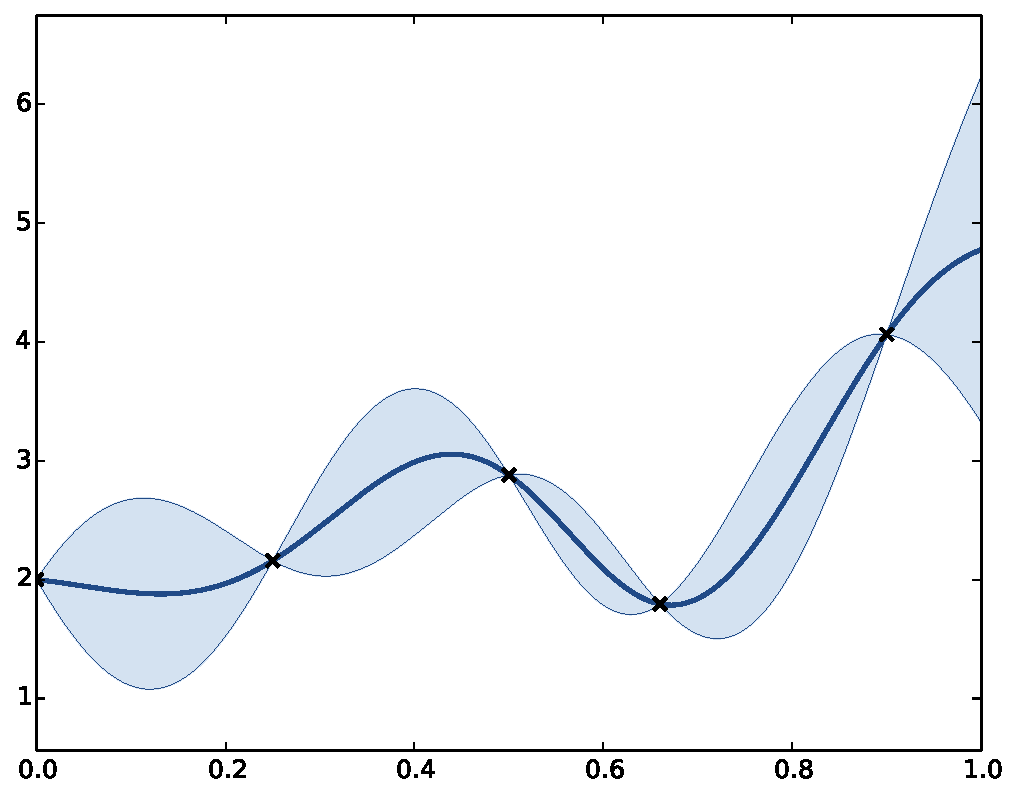
\includegraphics[height=5cm]{4_optimization/figures/python/ego_0}
\end{center}
\end{frame}

%%%%%%%%%%%%%%%%%%%%%%%%%%%%%%%%%%%%%%%%%%%%%%%%%%%%%%
\begin{frame}{}
In our example, the best observed value is 1.79
\begin{center}
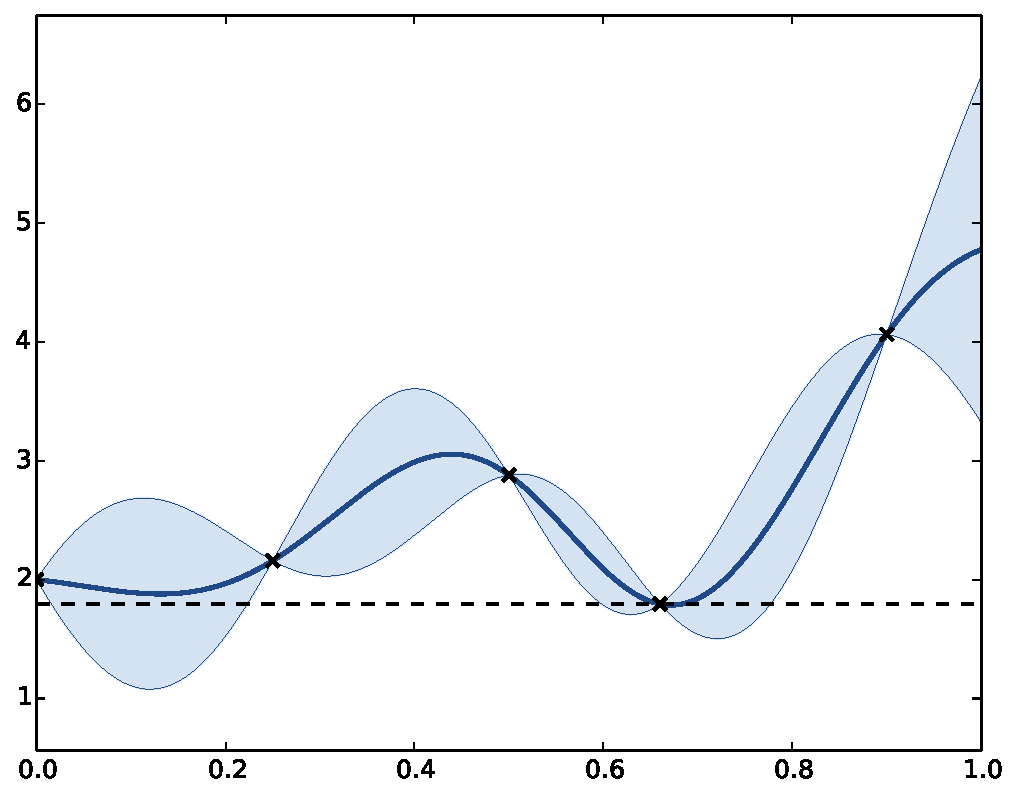
\includegraphics[height=5cm]{4_optimization/figures/python/ego_improv}
\end{center}
Various criteria can be studied
\begin{itemize}
	\item probability of improvement
	\item Expected improvement
\end{itemize}
\end{frame}

%%%%%%%%%%%%%%%%%%%%%%%%%%%%%%%%%%%%%%%%%%%%%%%%%%%%%%
\begin{frame}{}
\textbf{Probability of Improvement:}
$$PI(x) = cdf \left(\frac{\min(F) - m(x)}{\sqrt{(c(x,x))}} \right)$$
\begin{center}
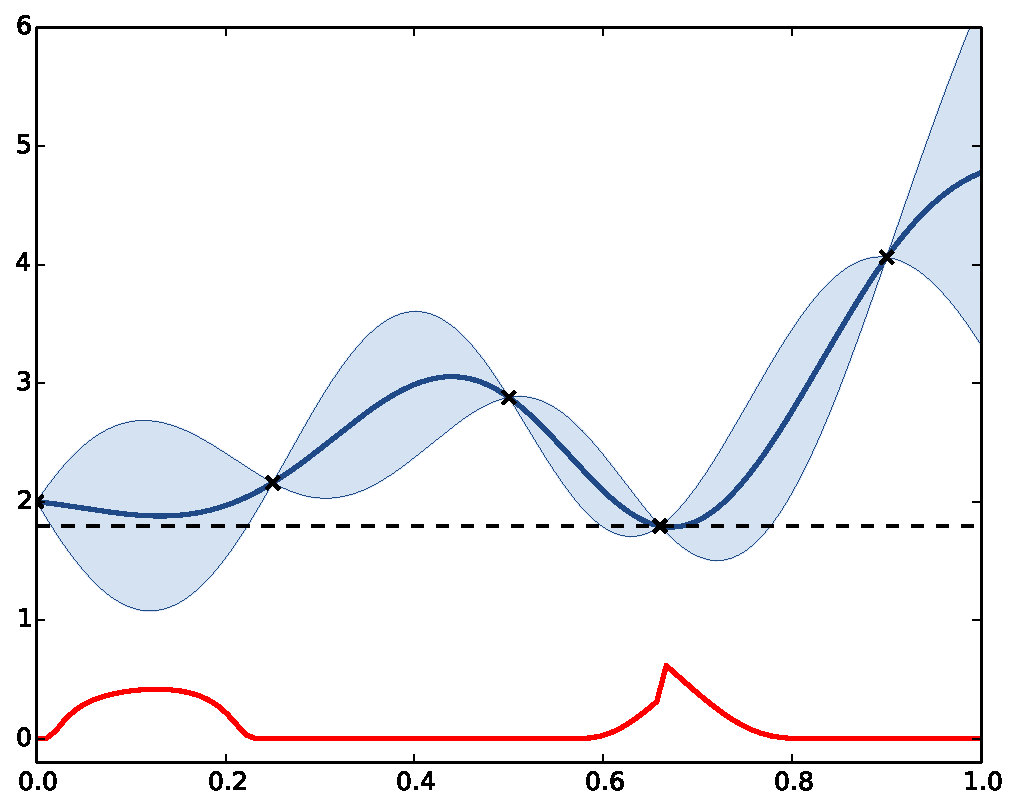
\includegraphics[height=5cm]{4_optimization/figures/python/ego_PI}
\end{center}
\end{frame}

%%%%%%%%%%%%%%%%%%%%%%%%%%%%%%%%%%%%%%%%%%%%%%%%%%%%%%
\begin{frame}{}
The point with the highest PI is often very close to the best observed value. We can show that there is a $x$ in the neighbourhood of $x^*$ such that $PI(x) \geq 0.5$.\\
\vspace{5mm}
For such points, the improvement cannot be large... \\
\vspace{3mm}
Can we find another criterion?
\end{frame}

%%%%%%%%%%%%%%%%%%%%%%%%%%%%%%%%%%%%%%%%%%%%%%%%%%%%%%
\begin{frame}{}
\textbf{Expected Improvement:}
\begin{equation*}
\begin{split}
E&I(x) =  \int_{-\infty}^{\min(F)} \max\left(0,Y(x)\right) ~dy(x) = \dots = \\
& \sqrt{c(x,x)} (u(x) cdf(u(x)) + pdf(u(x))) \quad \text{ with } u(x) = \frac{\min(F) - m(x)}{\sqrt{(c(x,x))}}
\end{split}
\end{equation*}
%\qquad with $ \displaystyle u(x) = \frac{\min(F) - m(x)}{\sqrt{(c(x,x))}}$
\begin{center}
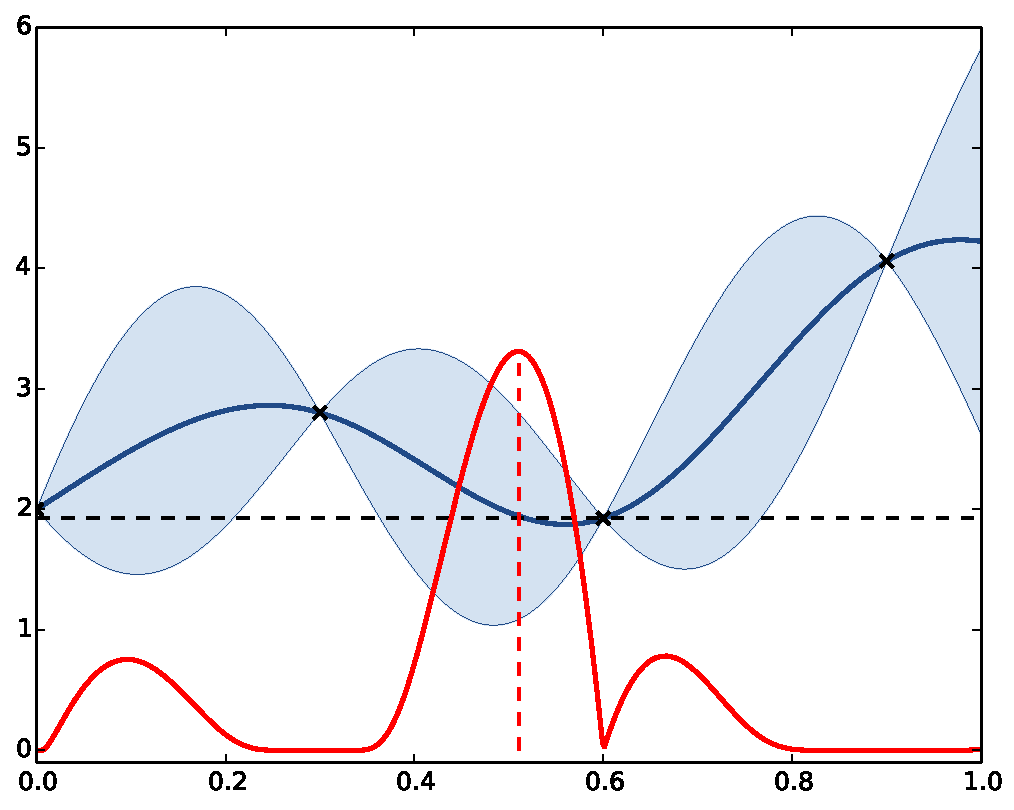
\includegraphics[height=5cm]{4_optimization/figures/python/ego_EI0}
\end{center}
\end{frame}

%%%%%%%%%%%%%%%%%%%%%%%%%%%%%%%%%%%%%%%%%%%%%%%%%%%%%%
\begin{frame}{Expected Improvement}
Let's see how it works... iteration 1
\begin{center}
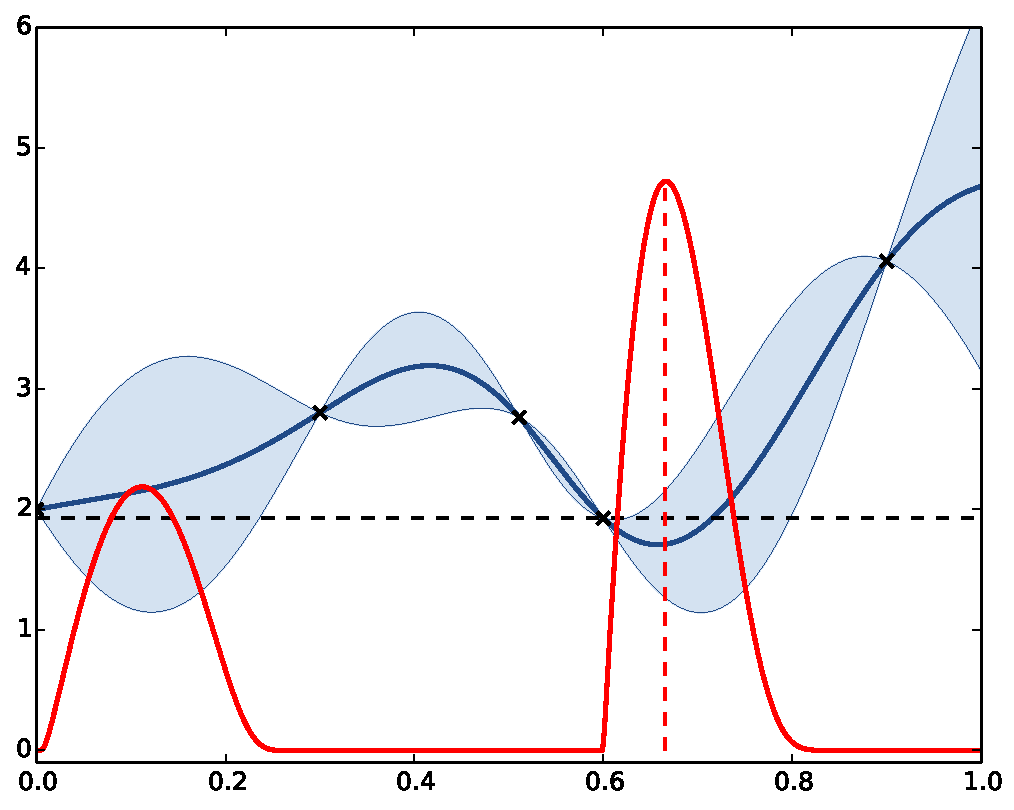
\includegraphics[height=5cm]{4_optimization/figures/python/ego_EI1}
\end{center}
\end{frame}

%%%%%%%%%%%%%%%%%%%%%%%%%%%%%%%%%%%%%%%%%%%%%%%%%%%%%%
\begin{frame}[noframenumbering]{Expected Improvement}
Let's see how it works... iteration 2
\begin{center}
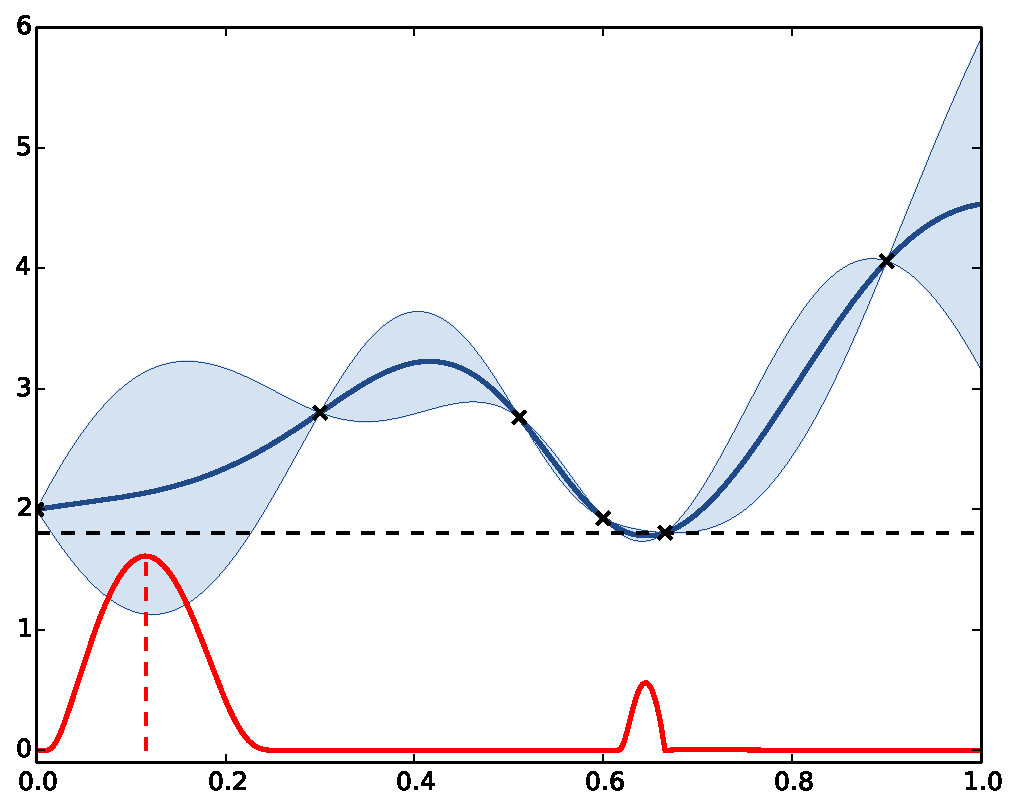
\includegraphics[height=5cm]{4_optimization/figures/python/ego_EI2}
\end{center}
\end{frame}

%%%%%%%%%%%%%%%%%%%%%%%%%%%%%%%%%%%%%%%%%%%%%%%%%%%%%%
\begin{frame}[noframenumbering]{Expected Improvement}
Let's see how it works... iteration 3
\begin{center}
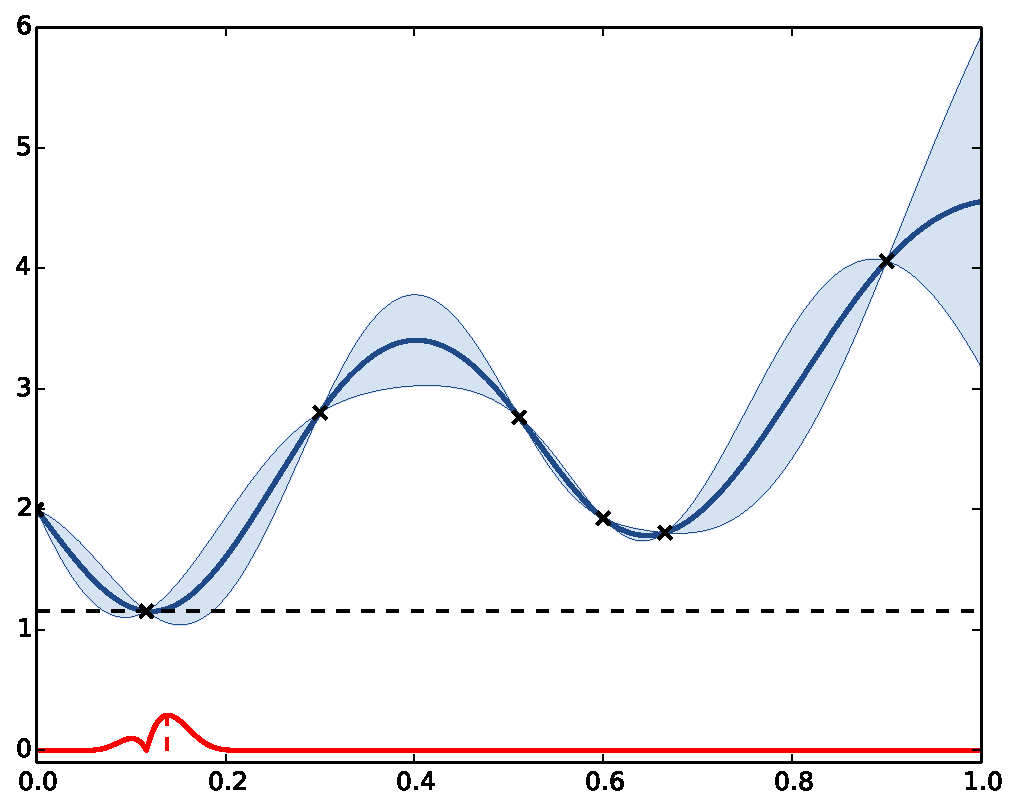
\includegraphics[height=5cm]{4_optimization/figures/python/ego_EI3}
\end{center}
\end{frame}

%%%%%%%%%%%%%%%%%%%%%%%%%%%%%%%%%%%%%%%%%%%%%%%%%%%%%%
\begin{frame}[noframenumbering]{Expected Improvement}
Let's see how it works... iteration 4
\begin{center}
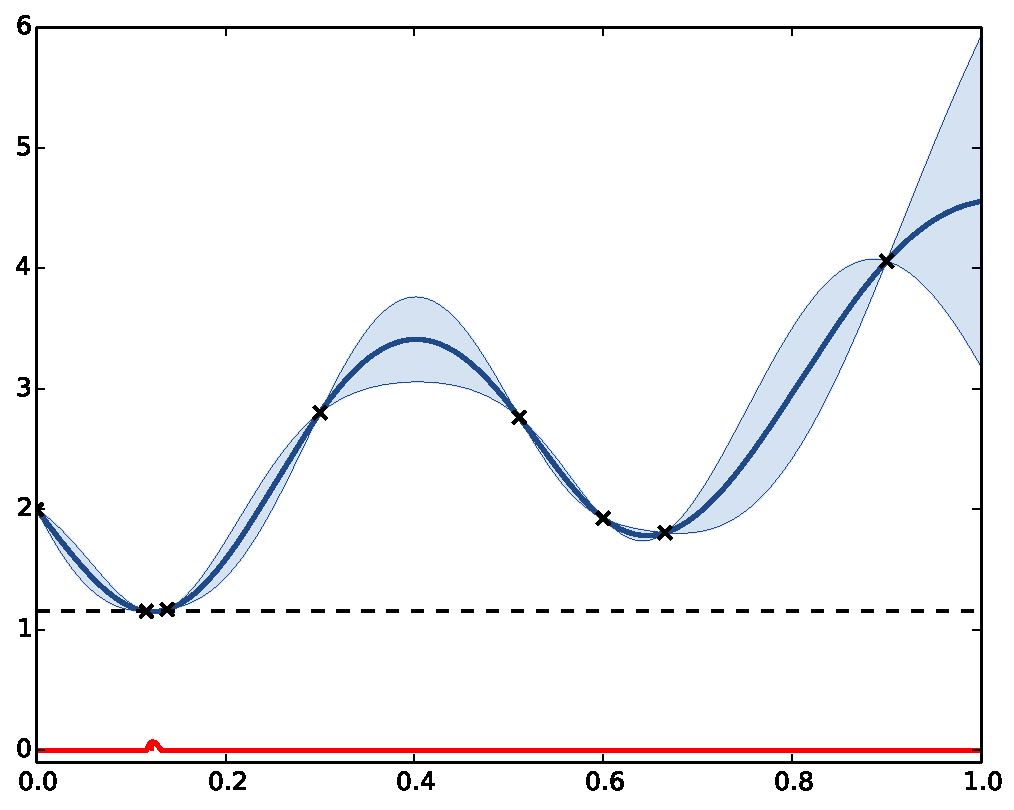
\includegraphics[height=5cm]{4_optimization/figures/python/ego_EI4}
\end{center}
\end{frame}

%%%%%%%%%%%%%%%%%%%%%%%%%%%%%%%%%%%%%%%%%%%%%%%%%%%%%%
\begin{frame}[noframenumbering]{Expected Improvement}
Let's see how it works... iteration 5
\begin{center}
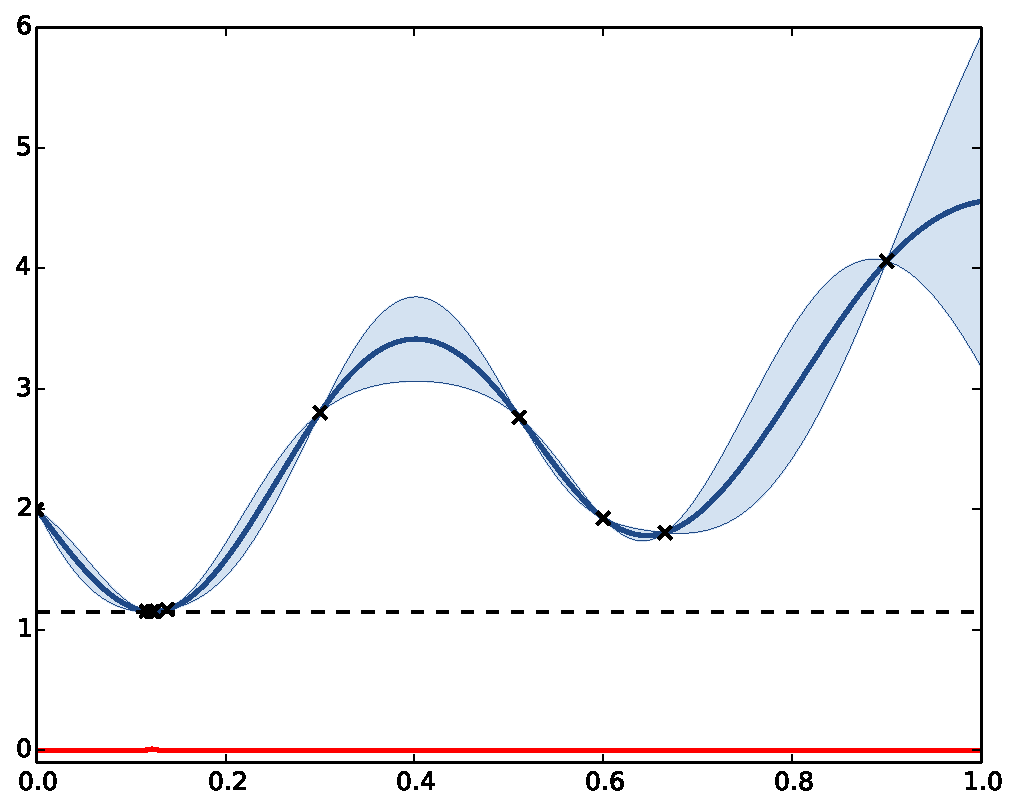
\includegraphics[height=5cm]{4_optimization/figures/python/ego_EI9}
\end{center}
\end{frame}

%%%%%%%%%%%%%%%%%%%%%%%%%%%%%%%%%%%%%%%%%%%%%%%%%%%%%%
\begin{frame}{Expected Improvement}
This algorithm is called \textbf{Efficient Global Optimization} (EGO, Jones et al., 1998):
\begin{enumerate}
	\item make an initial design of experiments $X$ and calculate the associated $F$, $t = \mathtt{length}(F)$
	\item built a GP from $(X,F)$ (max. log-likelihood on $\sigma$ and $\theta_i$'s)
	\item $X_{t+1}= \arg \max_x EI(x)$
	\item calculate $F_{t+1}=f(X_{t+1})$, increment $t$
	\item stop ($t>t^\text{max}$) or go to {\color{blue}2.}
\end{enumerate}
\vspace{5mm}
\begin{itemize}
	\item[+] EGO provides a good trade-off between exploitation and exploration without arbitrary parameters.
	\item[+] It requires few function observations (10 in the example) to get close to optimal regions.
\end{itemize}
%\begin{example}
%From the previous 5 iterations, we obtain $1.44e39$ for the conditioning of the covariance matrix. Eigenvalues are
%$$ (67.70,\  24.86,\  5.13,\  1.68,\  0.45,\  0.16,\  0.01,\  0.00,\  0.00,\ 0.00) $$
%\end{example}
\end{frame}

%%%%%%%%%%%%%%%%%%%%%%%%%%%%%%%%%%%%%%%%%%%%%%%%%%%%%%
%\begin{frame}{}
%\begin{exampleblock}{Illustration for $d=6$ (Hartman)}
%	Illustration in higher dimension
%\begin{center}
%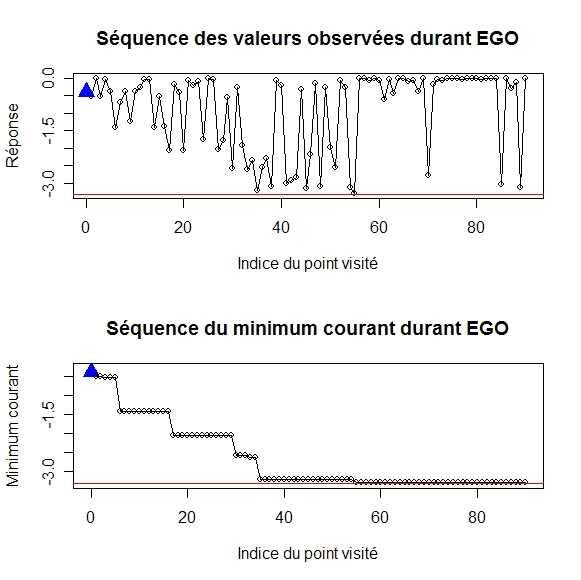
\includegraphics[height=5.5cm]{4_optimization/figures/egoHartman} 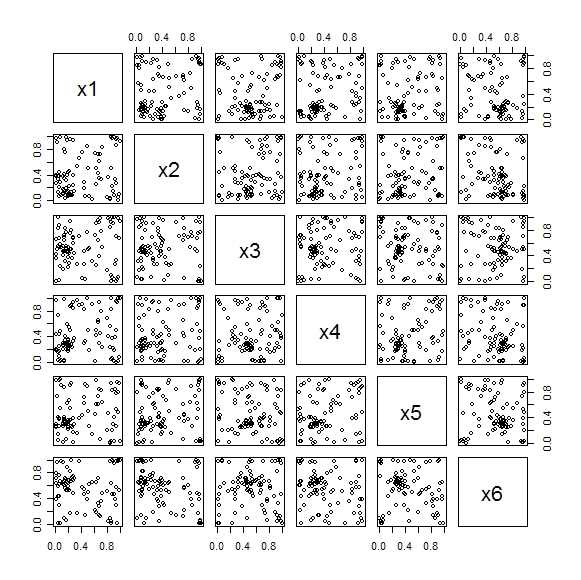
\includegraphics[height=5.5cm]{4_optimization/figures/egoHartman2}
%\end{center}
%\small Source: \textit{DiceOptim}, Roustant, Ginsbourger and Deville, 2009.
%\end{exampleblock}
%\end{frame}

%%%%%%%%%%%%%%%%%%%%%%%%%%%%%%%%%%%%%%%%%%%%%%%%%%%%%%
\begin{frame}{}
\begin{exampleblock}{Example in 5d: surface displacements misfit minimization}
$\Rightarrow$ demo with \texttt{mainInversionPunctualDisplSource.R}\\
!!! normalize the data: WLS has a few very large values, it is always $>0$: make it more gaussian, 
$\mathtt{wls}\_norm = \log(1+\mathtt{wls})$ and all $x$'s and $\mathtt{wls}\_norm$ between 0 and 1.
\begin{minipage}[c]{0.6\textwidth}
\begin{center}
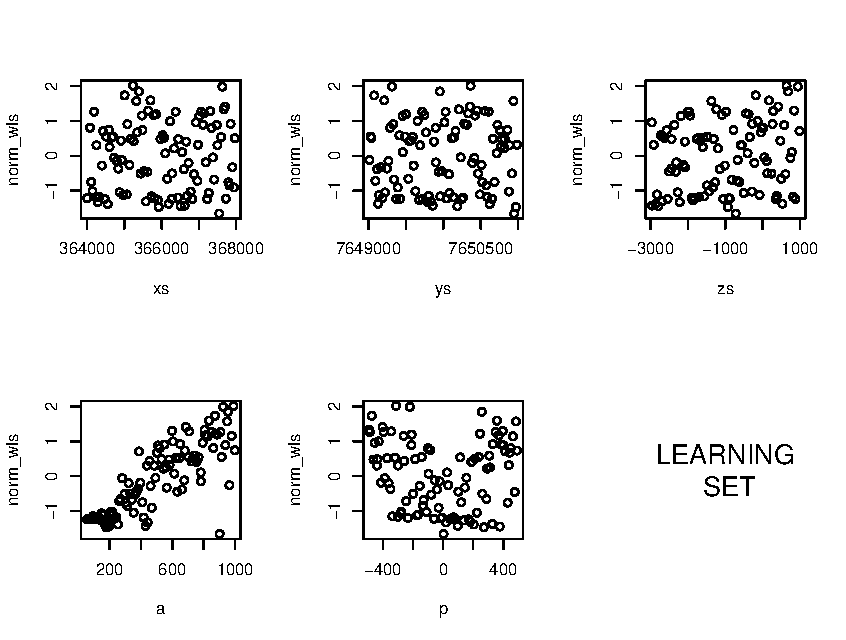
\includegraphics[width=\textwidth]{4_optimization/figures/misfit_learn_set} 
\end{center}
\end{minipage}
\hspace{0.3cm}
\begin{minipage}[c]{0.30\textwidth}
{\small 100 $\{xs,ys,zs,a,p\}$ points chosen through an optimized Latin Hypercube Sampling 
(\texttt{R} libraries \texttt{DiceDesign} or \texttt{lhs}).}\\
\end{minipage}
\end{exampleblock}
\end{frame}

%%%%%%%%%%%%%%%%%%%%%%%%%%%%%%%%%%%%%%%%%%%%%%%%%%%%%%
\begin{frame}{}
\small (demo with \texttt{mainInversionPunctualDisplSource.R}, cont.)
\begin{center}
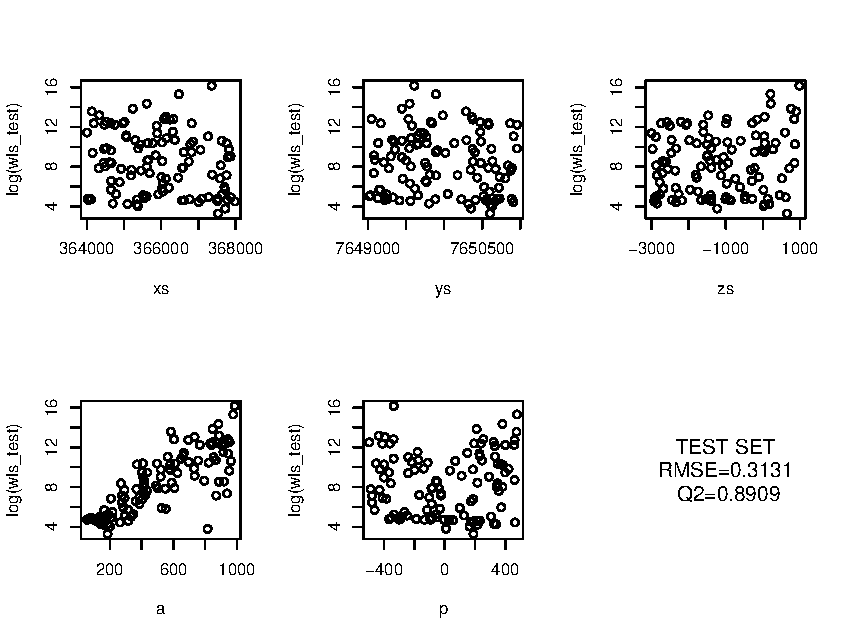
\includegraphics[width=0.7\textwidth]{4_optimization/figures/misfit_test_set} 
\end{center}
{\tiny 110 random $\{xs,ys,zs,a,p\}$ test points.}\\
\end{frame}

%%%%%%%%%%%%%%%%%%%%%%%%%%%%%%%%%%%%%%%%%%%%%%%%%%%%%%
\begin{frame}{}
\small (demo with \texttt{mainInversionPunctualDisplSource.R}, cont.)
\begin{center}
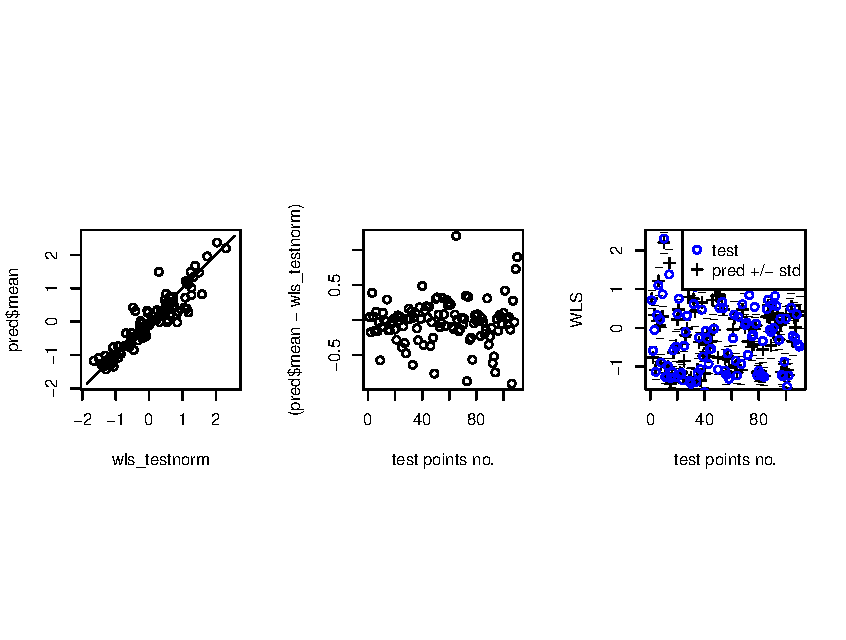
\includegraphics[width=0.9\textwidth]{4_optimization/figures/misfit_test_set_2} 
\end{center}
{\tiny 110 test points.}\\
\end{frame}

%%%%%%%%%%%%%%%%%%%%%%%%%%%%%%%%%%%%%%%%%%%%%%%%%%%%%%
\begin{frame}{}
\small (demo with \texttt{mainInversionPunctualDisplSource.R}, cont.)\\
\small EGO parameters: anisotropic Mat\`ern 5/2 kernel, GP updated (log-likelihood maximized) every 5 added points, BFGS with bounded variables (from \texttt{optim()} function) restarted from random initial points for maximizing log-likelihood and EI.
\begin{minipage}[c]{0.6\textwidth}
\begin{center}
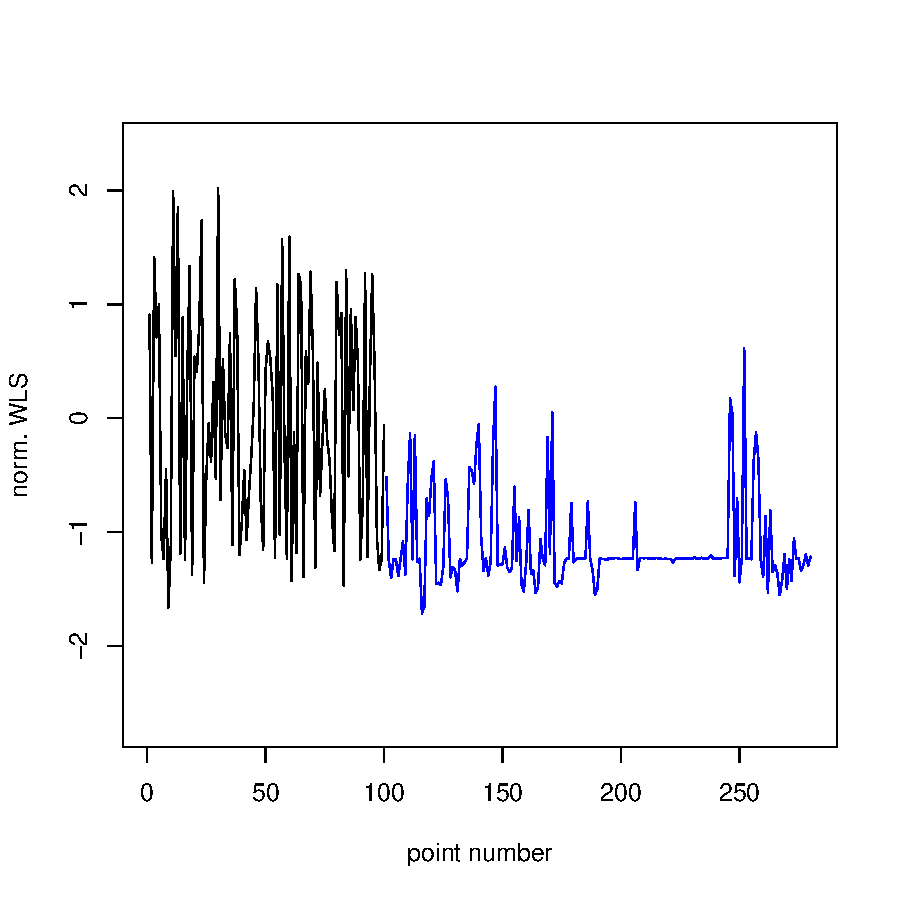
\includegraphics[width=\textwidth]{4_optimization/figures/misfit_EGO_conv} 
\end{center}
\end{minipage}
\hspace{0.3cm}
\begin{minipage}[c]{0.3\textwidth}
Preferential sampling of good regions of $S$, but global therefore sometimes increasing WLS.
Lower bound on $\theta_i$'s increased from 0.08 to 0.1 at $t=250$ ($x_i$'s and $\theta_i$'s
normed between 0 and 1).
\end{minipage}
\end{frame}

%%%%%%%%%%%%%%%%%%%%%%%%%%%%%%%%%%%%%%%%%%%%%%%%%%%%%%
\begin{frame}{}
\small (demo with \texttt{mainInversionPunctualDisplSource.R}, cont.)
\begin{minipage}[c]{0.6\textwidth}
\begin{center}
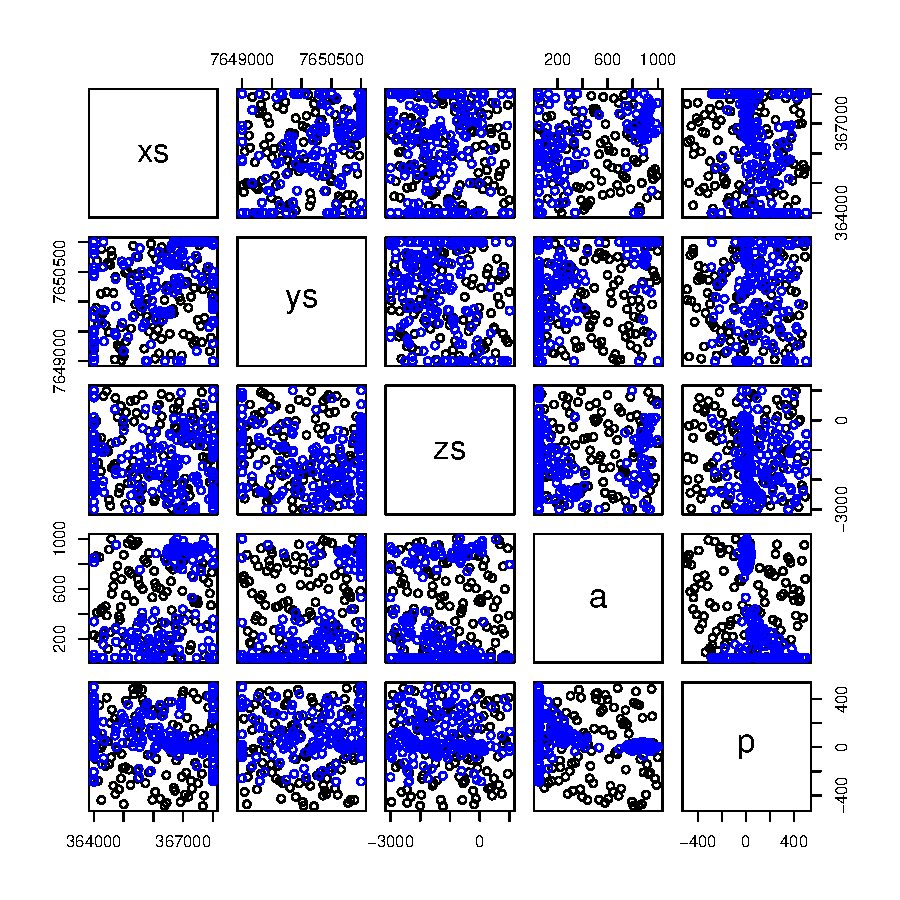
\includegraphics[width=\textwidth]{4_optimization/figures/pairs_X_old_new} 
\end{center}
\end{minipage}
\hspace{0.3cm}
\begin{minipage}[c]{0.3\textwidth}
Black: LHS initial points. \\
Blue: EGO points.\\
\vskip\baselineskip
Note the patterns in new points. Accumulation at lower bound of $a$ and mid interval of $p$ before $t=250$.
\end{minipage}
\end{frame}

%%%%%%%%%%%%%%%%%%%%%%%%%%%%%%%%%%%%%%%%%%%%%%%%%%%%%%
\begin{frame}{}
\small (demo with \texttt{mainInversionPunctualDisplSource.R}, cont.)
\begin{minipage}[c]{0.6\textwidth}
\begin{center}
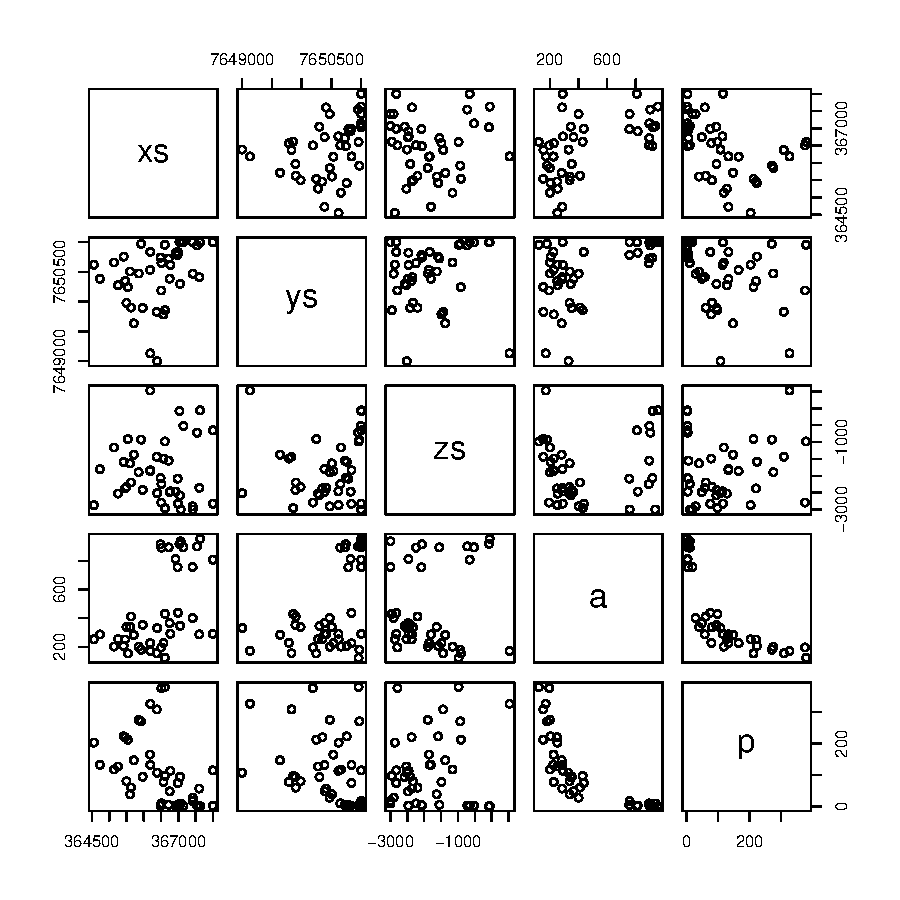
\includegraphics[width=\textwidth]{4_optimization/figures/pairs_X_good_15percent} 
\end{center}
\end{minipage}
\hspace{0.3cm}
\begin{minipage}[c]{0.3\textwidth}
15\% best sampled points. Note the ``function'' for the $(a,p)$ pair, i.e., $a^\star(p^\star)$.
\end{minipage}
\end{frame}

%%%%%%%%%%%%%%%%%%%%%%%%%%%%%%%%%%%%%%%%%%%%%%%%%%%%%%
\begin{frame}{}
\small (demo with \texttt{mainInversionPunctualDisplSource.R}, cont.)
\mbox{ % mbox to avoid linebreak
\begin{minipage}[c]{0.56\textwidth}
\begin{center}
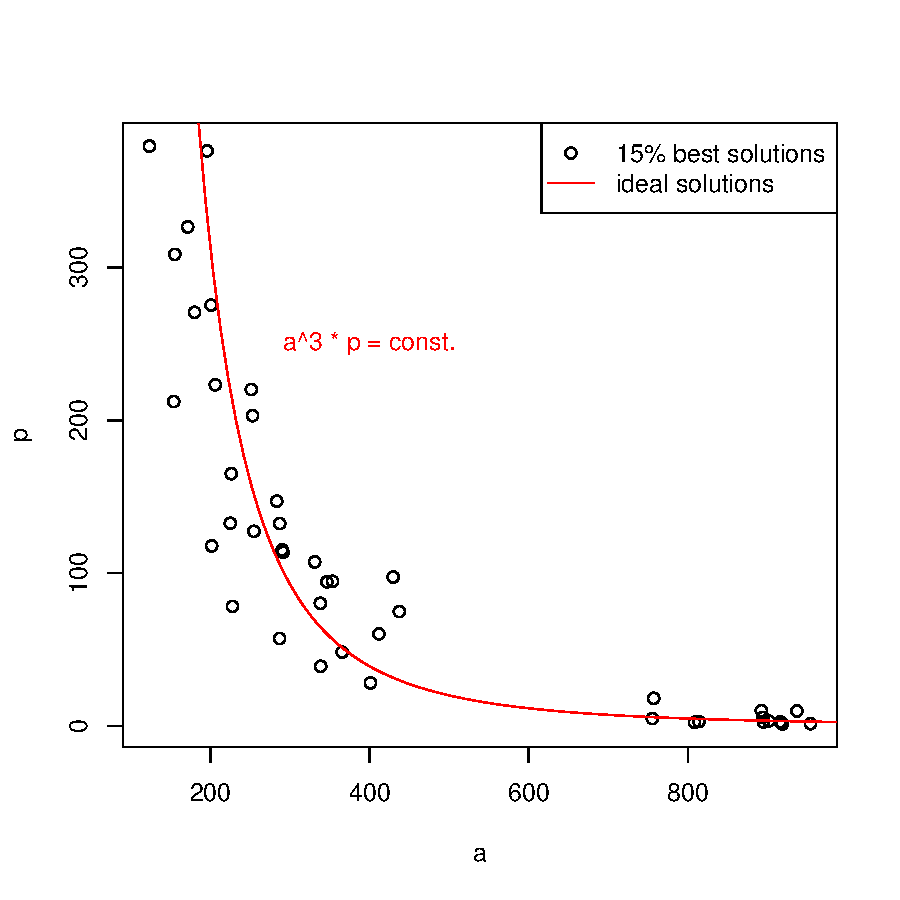
\includegraphics[width=\textwidth]{4_optimization/figures/non_identif_a_p} 
\end{center}
\end{minipage}
\hspace{0.3cm}
\begin{minipage}[c]{0.4\textwidth}
Mogi model only dependency in $a$ and $p$ is through $a^3 \times p$: it is not identifiable. \\
\vskip\baselineskip
EGO tells it by preferential sampling in the valley 
$$a^3 \times p = \text{const.} = {a^\star}^3 \times p^\star$$
\end{minipage}
} % end mbox
Other EGO output: a statistical model of WLS. \\
The last length scales are an indication of the 
sensitivity of WLS to each variable: $a$, $p$ and $zs$ are very sensitive 
($\theta_i$'s small, in $[0.08,0.1]$), $xs$ a little sensitive ($\theta \text{ in } [0.1,2.5]$) 
and $ys$ insensitive ($\theta \approx 3$).
\end{frame}

%%%%%%%%%%%%%%%%%%%%%%%%%%%%%%%%%%%%%%%%%%%%%%%%%%%%%%
\begin{frame}{}
\begin{exampleblock}{Difficulties and challenges with EGO}
\begin{itemize}
\item Standard GPs are limited to $n \approx 1000$ points (covariance matrix inversion).
\item EGO clusters points in good regions, the covariance matrix may become ill-conditionned 
if length scales $\theta_i$ are too large w.r.t. $X$.
\item Although the method perfectly applies to large dimensional spaces ($d>100$), larger $d$ 
may require larger $n$, back 2 lines above.
\item EGO does not converge in the traditional sense: it creates dense samples in the volume of $S$. 
The efficiency comes from the order in which points are sampled.
\end{itemize}
$\Rightarrow$ these are the topics of current research. Let's mention a few extensions next.
\end{exampleblock}
\end{frame}

%%%%%%%%%%%%%%%%%%%%%%%%%%%%%%%%%%%%%%%%%%%%%%%%%%%%%%
\begin{frame}{}
\begin{exampleblock}{EGO continuations}
\begin{itemize}
\item Parallelized EGO: estimate the $EI$ of groups of points, cf. Ginsbourger et al. 
\item Finite budget: $EI$ of a single $x$ is only optimal at the last iteration. Theory of dynamic $EI$, cf. Ginsbourger et al.
\item EGO and bad covariance matrix conditioning: replace points that are close-by by one point and the associated derivatives (cf. M. Osborn, L. Laurent), regularizations (cf. Le Riche et al.)
\item SUR strategies: (Step-wise Uncertainty Reduction), reduce the entropy of the optimum (cf. Vasquez et al.), or the average probability of incursions below $min(F)$ (cf. Picheny).
\end{itemize}
\end{exampleblock}
\end{frame}

%%%%%%%%%%%%%%%%%%%%%%%%%%%%%%%%%%%%%%%%%%%%%%%%%%%%%%
\begin{frame}{}
\begin{exampleblock}{Related problems addressed with GPs}
\begin{itemize}
\item EGO with constraints: $\min_x f(x) \text{ s.t. } g(x) \le 0$, multiply the $EI$ by the probability of constraints satisfaction.
\item GP for target attainment: find the set of $x$ s.t. $f(x) = T$, change the $EI$ into $c(x,x) \times \text{pdf}\left((T-m(x))/sqrt(c(x,x))\right)$, cf. Picheny et al.
\item GP for probability estimation: find $\mathds P (f(x,U)\le T) $ where $U$ is a random vector.
\item GP for multi-objective optimization: $\min_x \{f_1(x), \dots f_m(x)\}$, cf. Binois et al.
\end{itemize}
\end{exampleblock}
\end{frame}

%%%%%%%%%%%%%%%%%%%%%%%%%%%%%%%%%%%%%%%%%%%%%%%%%%%%%%%
%\begin{frame}{}
%One way to improve the conditioning of the covariance matrix is to replace two values that are close-by by one function value and one derivative:
%\begin{center}
%  \begin{tabular}{ccc}
%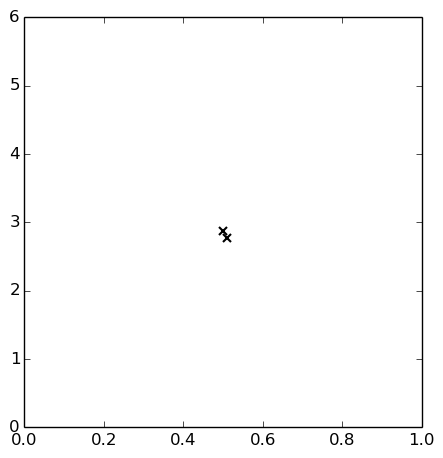
\includegraphics[height=4cm]{4_optimization/figures/python/osborn0} &
%
\includegraphics[height=4cm]{4_optimization/figures/Rightarrow} &
%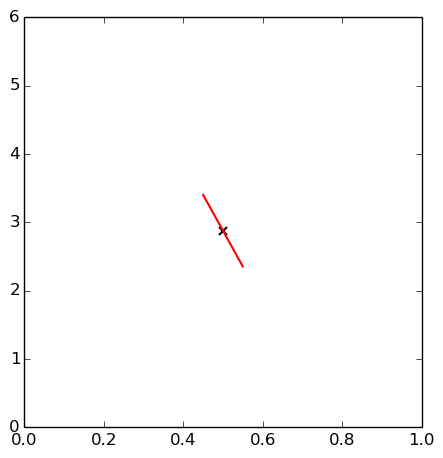
\includegraphics[height=4cm]{4_optimization/figures/python/osborn1} \\
%Cond. = 3842 & & Cond. = 10
%  \end{tabular}
%\end{center}
%This can be generalised to higher orders \alert{$\rightarrow$} Taylor expansion\\
%\small see articles from M. Osborn
%\end{frame}

%%%%%%%%%%%%%%%%%%%%%%%%%%%%%%%%%%%%%%%%%%%%%%%%%%%%%%%
%\begin{frame}{}
%If we know the computational budget in advance, adding new points at the \textbf{best one step ahead location} is not optimal.\\
%\vspace{5mm}
%Some improvements have been made toward this
%\begin{itemize}
%	\item Batch EGO
%	\item Parallelization of the algorithm
%\end{itemize}
%\vspace{5mm}
%\small see works from D. Ginsbourger
%\end{frame}

%%%%%%%%%%%%%%%%%%%%%%%%%%%%%%%%%%%%%%%%%%%%%%%%%%%%%%
%%%%%%%%%%%%%%%%%%%%%%%%%%%%%%%%%%%%%%%%%%%%%%%%%%%%%%
\section[Robust optim.]{Robust optimization}
\subsection{}

%%%%%%%%%%%%%%%%%%%%%%%%%%%%%%%%%%%%%%%%%%%%%%%%%%%%%%%
%\begin{frame}{}
%Robust optimization may mean various things:
%\begin{itemize}
%	\item There is observation noise on the output
%	\item Some input variables $U$ are uncertain
%	\item Model is uncertain, $f(x,U)$
%\end{itemize}
%\vspace{2mm}
%\begin{example}
%\begin{columns}[c]
%\column{3cm}
%	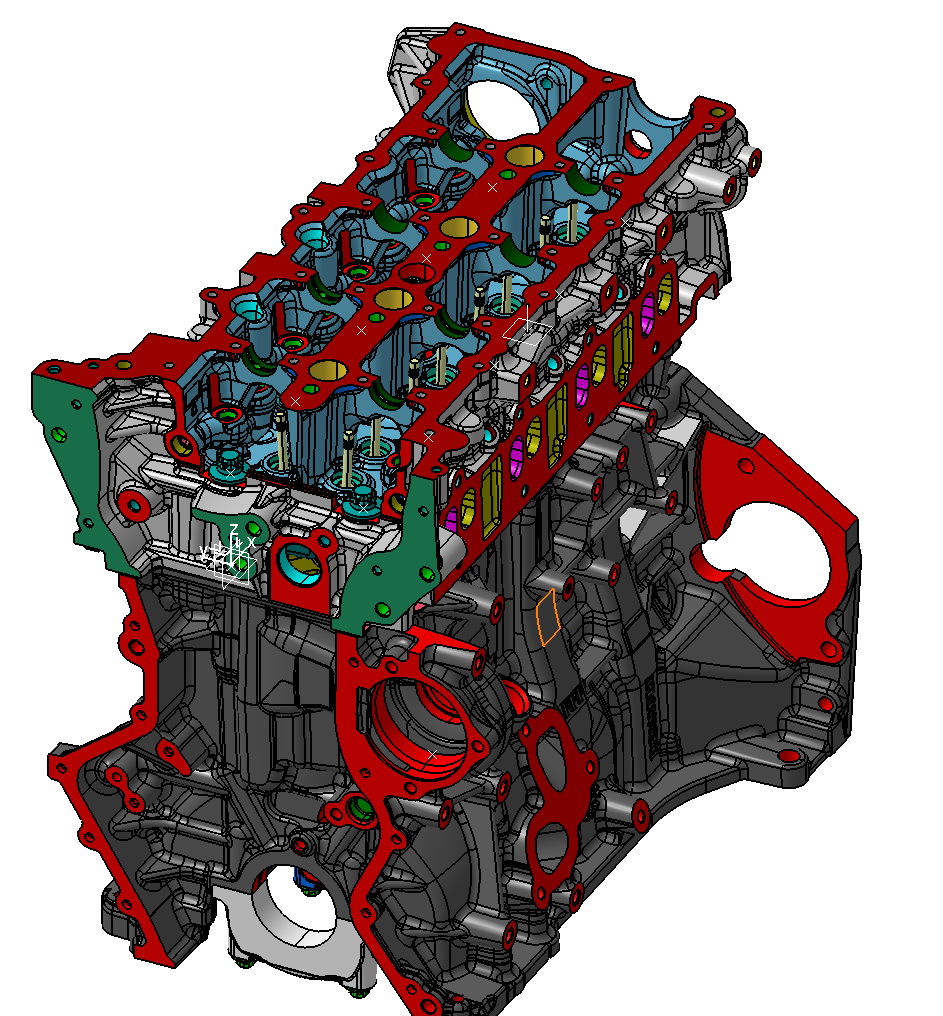
\includegraphics[height=4cm]{4_optimization/figures/RLRrobust}
%\column{5cm}
%	a +/- 1mm dispersion in the manufacturing of a car cylinder head  can degrade its performance (g CO2/km) by -20\% (worst case)\\
%\end{columns}
%\vspace{3mm}
%	\small Source: Talk from R. Le Riche at the Porquerolles Summer School, 2014
%\end{example}
%\end{frame}

%%%%%%%%%%%%%%%%%%%%%%%%%%%%%%%%%%%%%%%%%%%%%%%%%%%%%%
%\begin{frame}{}
% \begin{example}
% Here is a basic example:
% \begin{center}
% 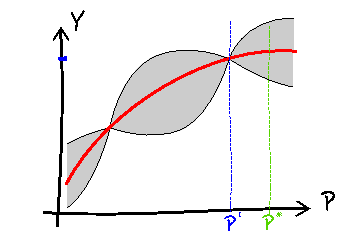
\includegraphics[height=5cm]{4_optimization/figures/optim_rob_a}\\
% Which input is the best?
% \end{center}
% \end{example}
% \end{frame}

%% %%%%%%%%%%%%%%%%%%%%%%%%%%%%%%%%%%%%%%%%%%%%%%%%%%%%%%
%% \begin{frame}[noframenumbering]{}
%\begin{example}
%Here is a basic example:
%\begin{center}
%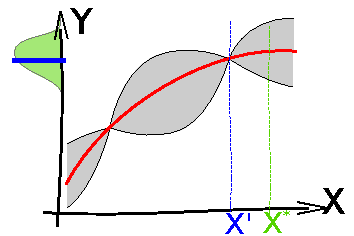
\includegraphics[height=5cm]{4_optimization/figures/optim_rob_b}\\
%Which input is the best?
%\end{center}
%\end{example}
%\end{frame}

%%%%%%%%%%%%%%%%%%%%%%%%%%%%%%%%%%%%%%%%%%%%%%%%%%%%%%%
%\begin{frame}[noframenumbering]{}
%\begin{example}
%A non Gaussian example
%\begin{center}
%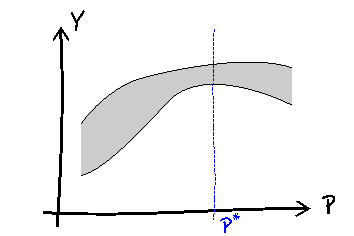
\includegraphics[height=5cm]{4_optimization/figures/optim_rob_c}\\
%In some cases, we may want to optimize the worst case scenario.
%\end{center}
%\end{example}
%\end{frame}

%%%%%%%%%%%%%%%%%%%%%%%%%%%%%%%%%%%%%%%%%%%%%%%%%%%%%%
\begin{frame}{}
Can EGO be adapted when observations are noisy?\\
\vspace{5mm}
First of all, using the current best observation as a minimum does not make much sense...\\
\vspace{5mm}
Some solutions are
\begin{itemize}
	\item[S1] Build a new model that interpolates $m(X)$ at $X$ where $m(X)$ accounts for the noise (non interpolating GP, e.g. with a white noise part in the kernel).
	\item[S2] Include observation noise and replace $\min(F)$ by $\min(m(X))$ in the EI expression
	\item[S3] Similar to 2 but consider an Expected Mean Improvement (V. Picheny).
\end{itemize}
\end{frame}

%%%%%%%%%%%%%%%%%%%%%%%%%%%%%%%%%%%%%%%%%%%%%%%%%%%%%%
\begin{frame}{Solution 1}
iteration 0
\begin{center}
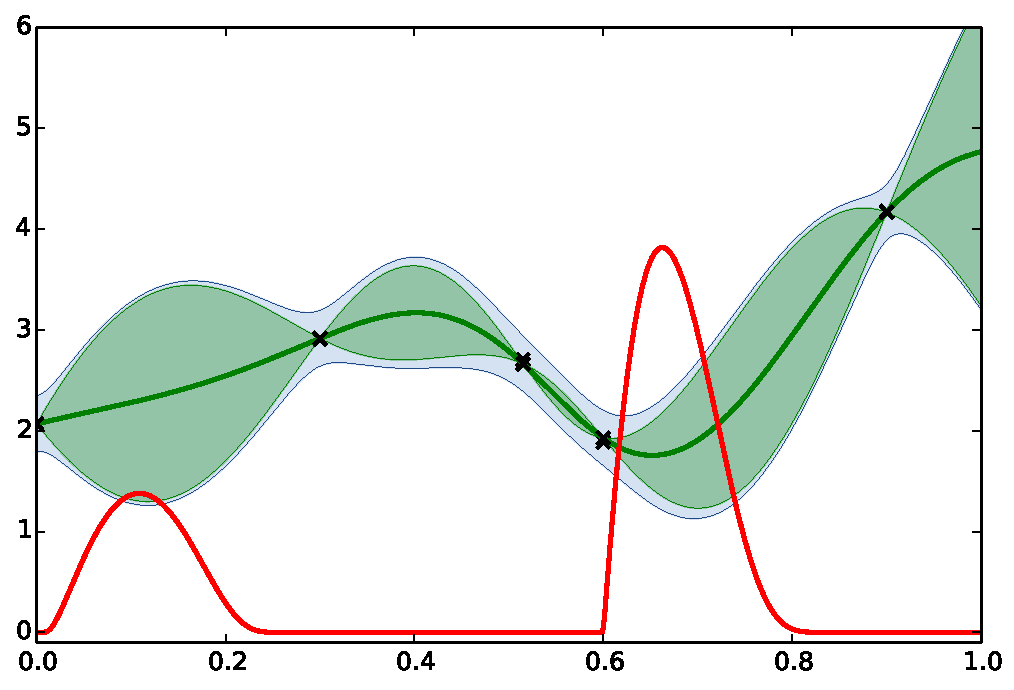
\includegraphics[height=5cm]{4_optimization/figures/python/ego_EI1n0}
\end{center}
\tiny (noisy observations and their denoised versions are both shown as black crosses)\\
\end{frame}

%%%%%%%%%%%%%%%%%%%%%%%%%%%%%%%%%%%%%%%%%%%%%%%%%%%%%%
\begin{frame}[noframenumbering]{Solution 1}
iteration 1
\begin{center}
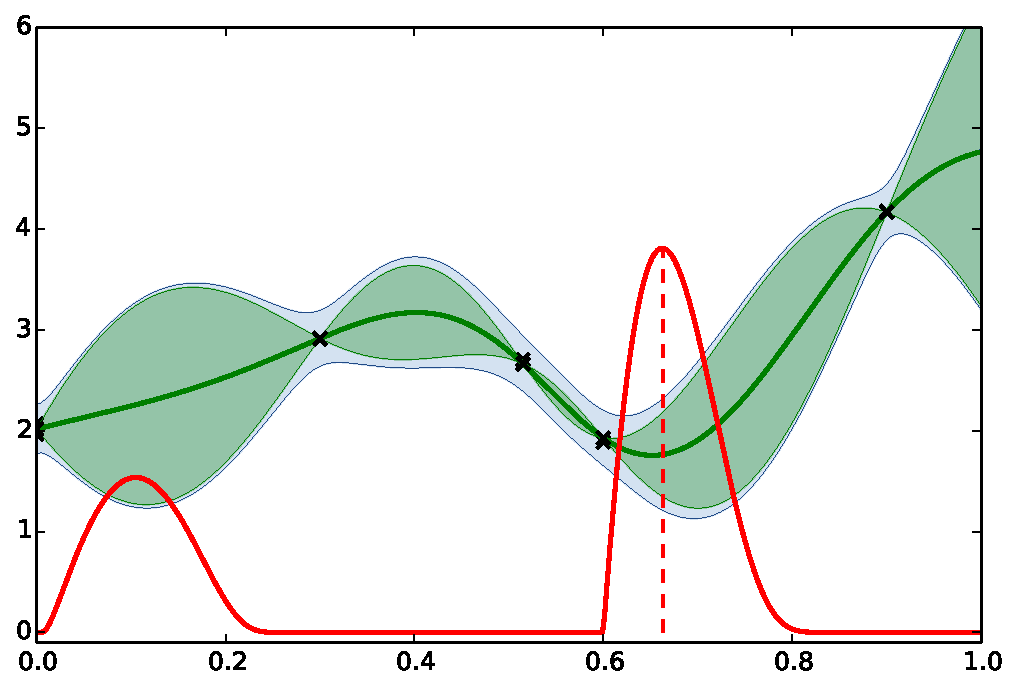
\includegraphics[height=5cm]{4_optimization/figures/python/ego_EI1n1}
\end{center}
\tiny (noisy observations and their denoised versions are both shown as black crosses)\\
\end{frame}

%%%%%%%%%%%%%%%%%%%%%%%%%%%%%%%%%%%%%%%%%%%%%%%%%%%%%%
\begin{frame}[noframenumbering]{Solution 1}
iteration 2
\begin{center}
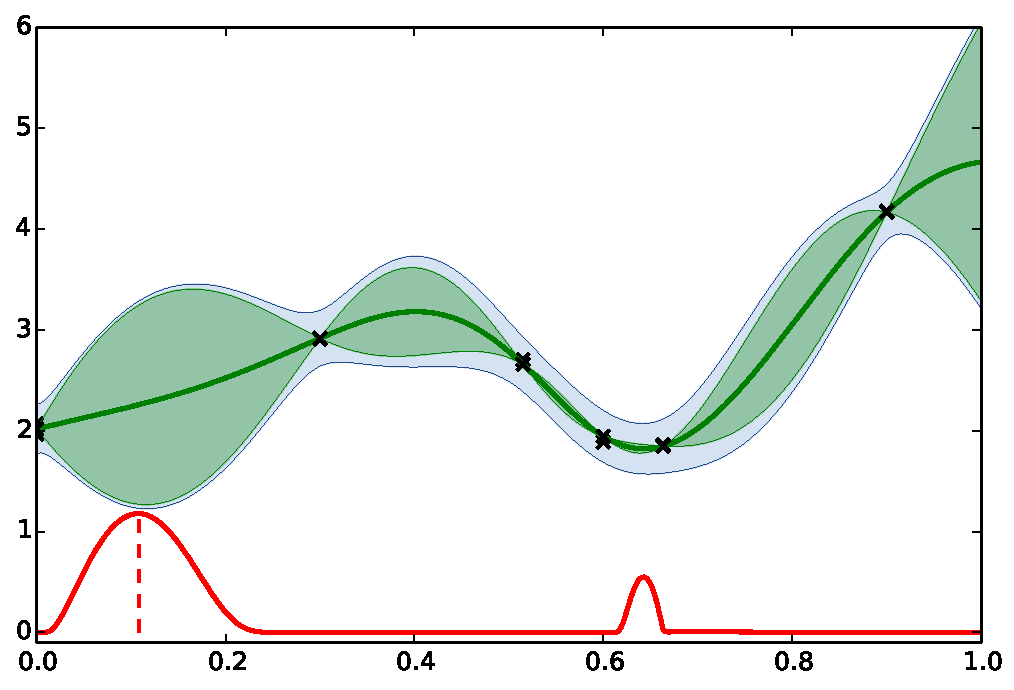
\includegraphics[height=5cm]{4_optimization/figures/python/ego_EI1n2}
\end{center}
\tiny (noisy observations and their denoised versions are both shown as black crosses)\\
\end{frame}

%%%%%%%%%%%%%%%%%%%%%%%%%%%%%%%%%%%%%%%%%%%%%%%%%%%%%%
\begin{frame}[noframenumbering]{Solution 1}
iteration 3
\begin{center}
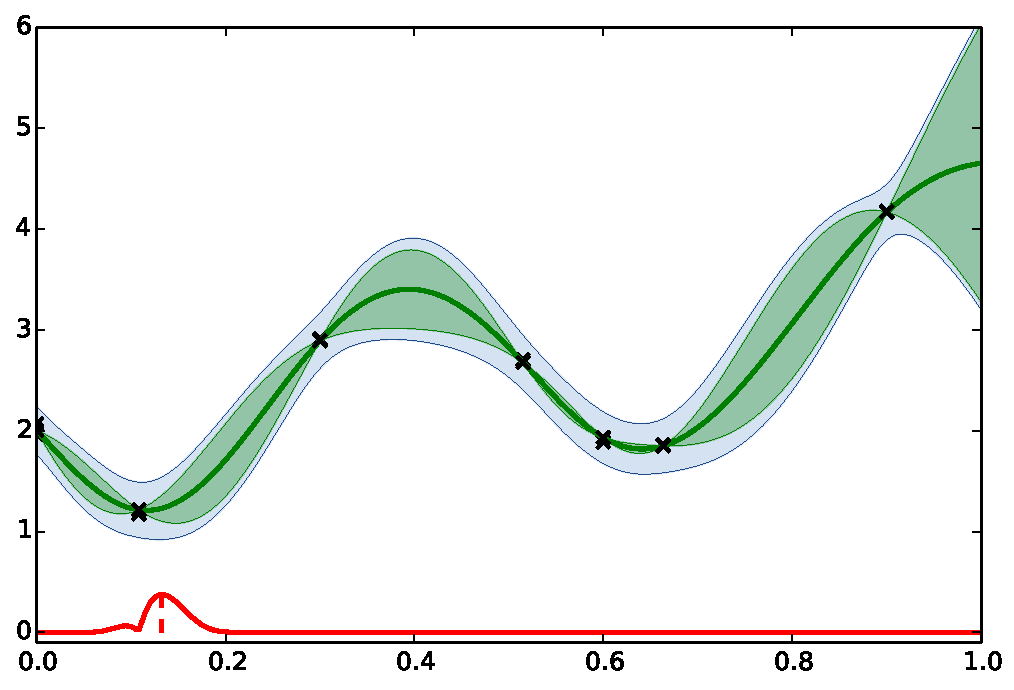
\includegraphics[height=5cm]{4_optimization/figures/python/ego_EI1n3}
\end{center}
\tiny (noisy observations and their denoised versions are both shown as black crosses)\\
\end{frame}

%%%%%%%%%%%%%%%%%%%%%%%%%%%%%%%%%%%%%%%%%%%%%%%%%%%%%%
\begin{frame}[noframenumbering]{Solution 1}
iteration 4
\begin{center}
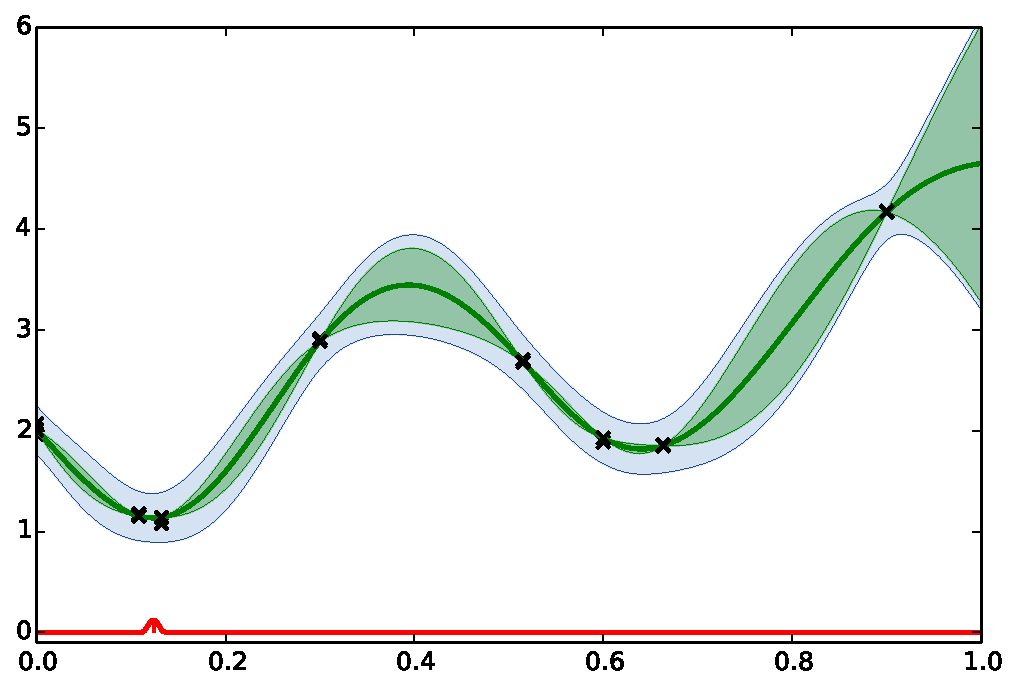
\includegraphics[height=5cm]{4_optimization/figures/python/ego_EI1n4}
\end{center}
\tiny (noisy observations and their denoised versions are both shown as black crosses)\\
\end{frame}

%%%%%%%%%%%%%%%%%%%%%%%%%%%%%%%%%%%%%%%%%%%%%%%%%%%%%%%
%%%%%%%%%%%%%%%%%%%%%%%%%%%%%%%%%%%%%%%%%%%%%%%%%%%%%%%
%\section[Related problems]{Related problems}
%\subsection{}

%%%%%%%%%%%%%%%%%%%%%%%%%%%%%%%%%%%%%%%%%%%%%%%%%%%%%%%
%\begin{frame}{}
%Some related optimization problems are:
%\begin{itemize}
%	\item calibration problems
%	\item probability computations
%\end{itemize}
%\vspace{8mm}
%Some algorithms with an EGO spirit can be applied:
%\begin{itemize}
% 	\item SUR methods
% \end{itemize}
%\end{frame}

%%%%%%%%%%%%%%%%%%%%%%%%%%%%%%%%%%%%%%%%%%%%%%%%%%%%%%%
%\begin{frame}{}
%We want to find the input(s) such that f(x) = 3.2
%\begin{center}
%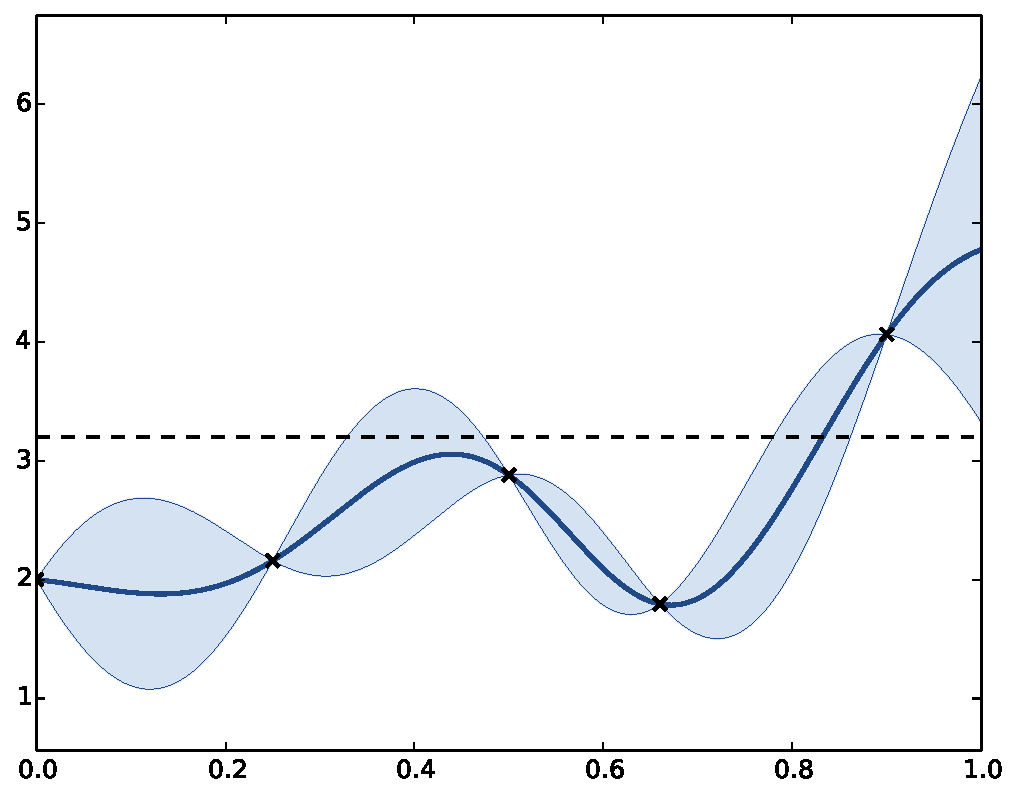
\includegraphics[height=5cm]{4_optimization/figures/python/inv}
%\end{center}
%\end{frame}

%%%%%%%%%%%%%%%%%%%%%%%%%%%%%%%%%%%%%%%%%%%%%%%%%%%%%%%
%\begin{frame}[noframenumbering]{}
%iteration 0:
%\begin{center}
%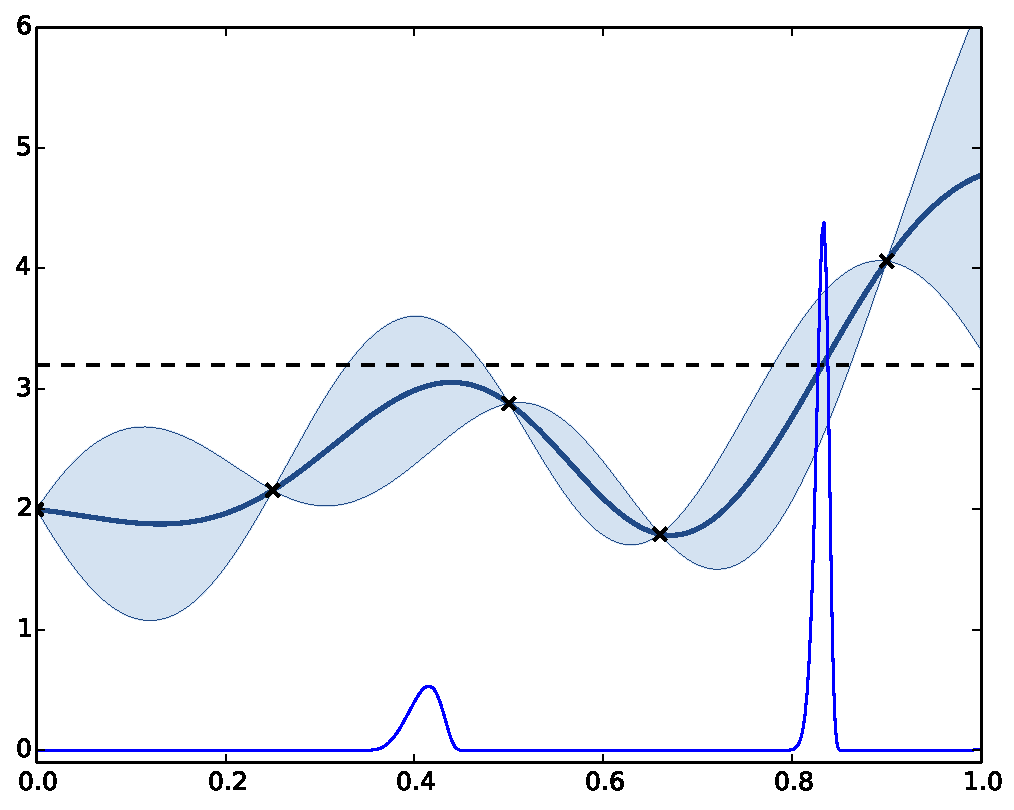
\includegraphics[height=5cm]{4_optimization/figures/python/invproba}
%\end{center}
%\end{frame}

%%%%%%%%%%%%%%%%%%%%%%%%%%%%%%%%%%%%%%%%%%%%%%%%%%%%%%%
%\begin{frame}[noframenumbering]{}
%iteration 1:
%\begin{center}
%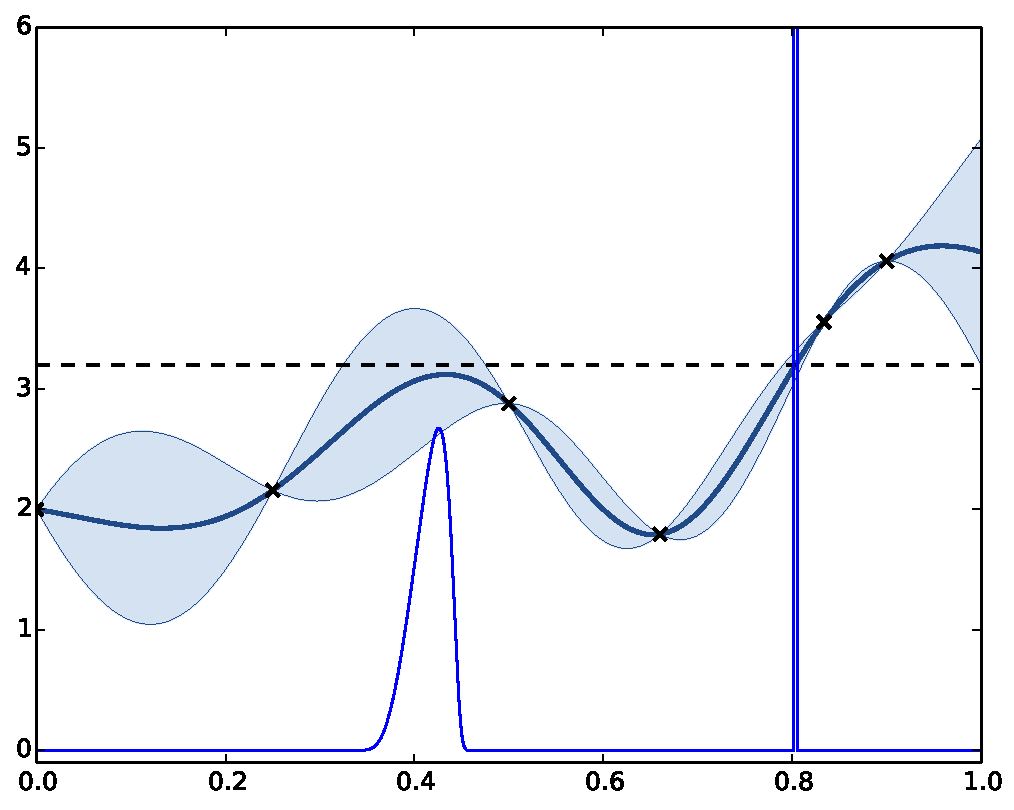
\includegraphics[height=5cm]{4_optimization/figures/python/invproba1}
%\end{center}
%\end{frame}

%%%%%%%%%%%%%%%%%%%%%%%%%%%%%%%%%%%%%%%%%%%%%%%%%%%%%%%
%\begin{frame}[noframenumbering]{}
%iteration 2:
%\begin{center}
%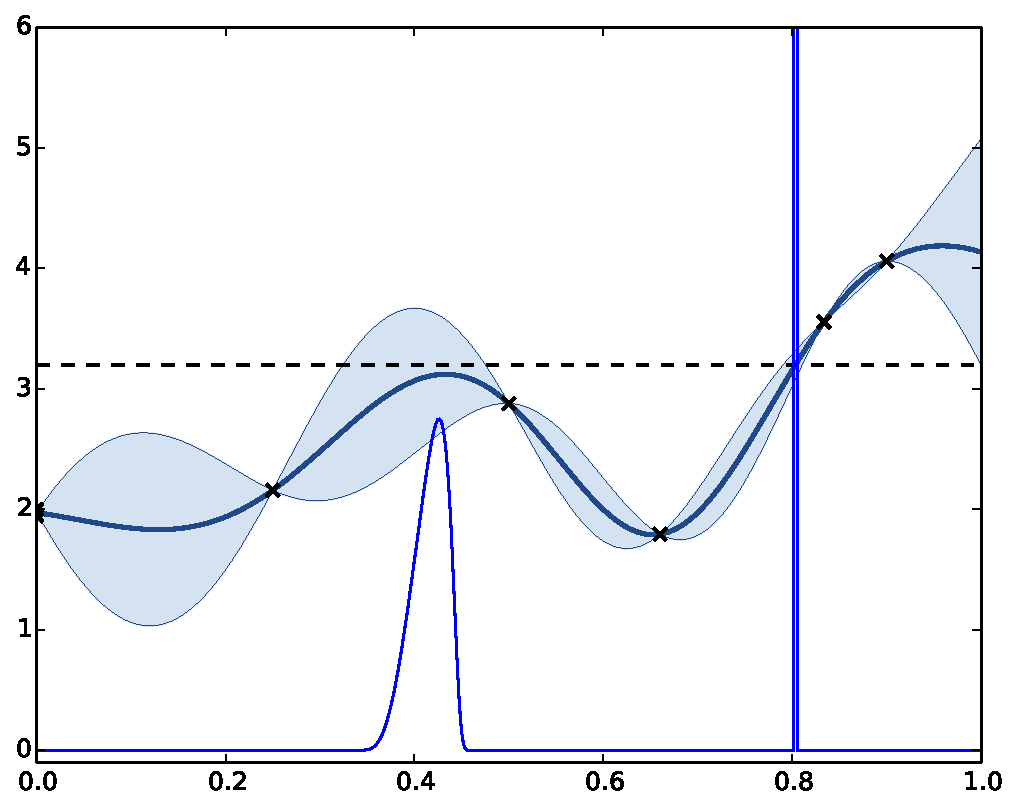
\includegraphics[height=5cm]{4_optimization/figures/python/invproba2}
%\end{center}
%\end{frame}

%%%%%%%%%%%%%%%%%%%%%%%%%%%%%%%%%%%%%%%%%%%%%%%%%%%%%%%
%\begin{frame}[noframenumbering]{}
%iteration 3:
%\begin{center}
%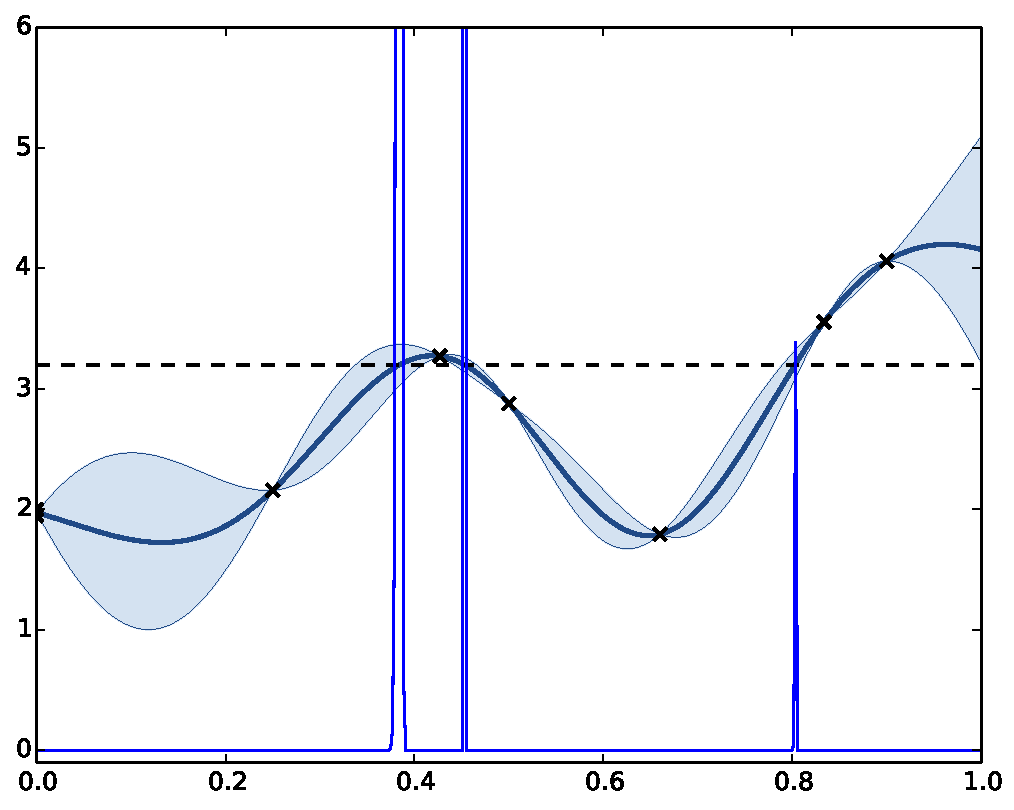
\includegraphics[height=5cm]{4_optimization/figures/python/invproba3}
%\end{center}
%\end{frame}

